\documentclass[12pt]{article}

% Packages for customizing title page
\usepackage{titling}
\usepackage{graphicx}

\usepackage[margin=.75in]{geometry} 

\usepackage{setspace}
\usepackage{subfigure}

\usepackage{graphicx} % For including images
\usepackage[margin=.75in]{geometry} % Set 1-inch margins
\usepackage{caption}


% Title page information
\title{The Susceptible-Infected-Recovered (SIR) Model}
\author{Ella Xu}
\date{\today}
\onehalfspacing
\begin{document}

\newgeometry{margin=4cm} % Adjust margin value as needed

\begin{titlepage}
    \begin{center}
    \vspace*{1cm}
    {\LARGE \textbf{\thetitle} \par}
    \vspace{1.5cm}
    {\Large \theauthor \par}
    \Large Computational Systems Biology Final Project \\
    \Large The University of Vermont \\
    \vspace{0.5cm}
    {\large \thedate \par}
    \end{center}
    \vspace*{1cm}
    \section*{Abstract}
    The classical Susceptible-Infected-Recovered (SIR) model provides a framework for analyzing the spread of infectious diseases within a closed population. This computational analysis simulates the model using ordinary differential equations to investigate how disease dynamics evolve over time under different transmission rates. Parameters analyzed include the transmission rate \(\beta\), recovery rate \(\gamma\), and basic reproduction number \(R_0\) to assess how they affect a possible outbreak. Limitations of the classical model are discussed, and future analyses taking into account demography, stochastic effects, and nonuniform population interactions to model the dynamics of more realistic epidemic behavior are suggested.
\end{titlepage}


% Add table of contents
%\tableofcontents

\restoregeometry


\newpage

\section*{Background}

The Susceptible-Infected-Recovered (SIR) model is an infectious epidemic model that can be applied in the context of disease spreading in a population. The SIR model assumes a simple closed population (no births, deaths, migration) and simple disease (no mutations or other ways to spread). The model originates from the work of Kermack and McKendrick in their 1927 paper, \textit{A Contribution to the Mathematical Theory of Epidemics}, where they proposed a general model for disease dynamics. The SIR model came about as a special case of their framework where transmission and recovery rates are constant. The model divides the population in three categories:

\begin{itemize}
  \item Susceptible (\(S\)) - people who have not yet been infected
  \item Infected (\(I\)) - currently sick and can transmit the disease to susceptible individuals
  \item Recovered (\(R\)) - individuals who have stopped being infected
\end{itemize}

The model simulates how an infectious disease propagates and eventually dies out in a closed population.

\newpage
\section*{Results and Methods}

Using the system of ordinary differential equations for the model published by Kermack and McKendrick (1927), we can show how the number of people in each category change with respect to time:

\[ \frac{dS}{dt} = -\frac{\beta}{N} SI\]
\[ \frac{dI}{dt} = \frac{\beta}{N} SI - \gamma I\]
\[\frac{dR}{dt} = \gamma I\]

Where:

\begin{itemize}
\item \(N\) is the total population size assumed constant,
\item \(\beta\) is the transmission rate that describes how likely a person is to get infected
\item \(\gamma\) is the recovery rate, the fraction of infectious individuals who recover each day. (i.e. if a person is infectious for 4 days, \(\gamma = 1/4\))
\end{itemize}

\begin{figure}[h!]
        \centering
        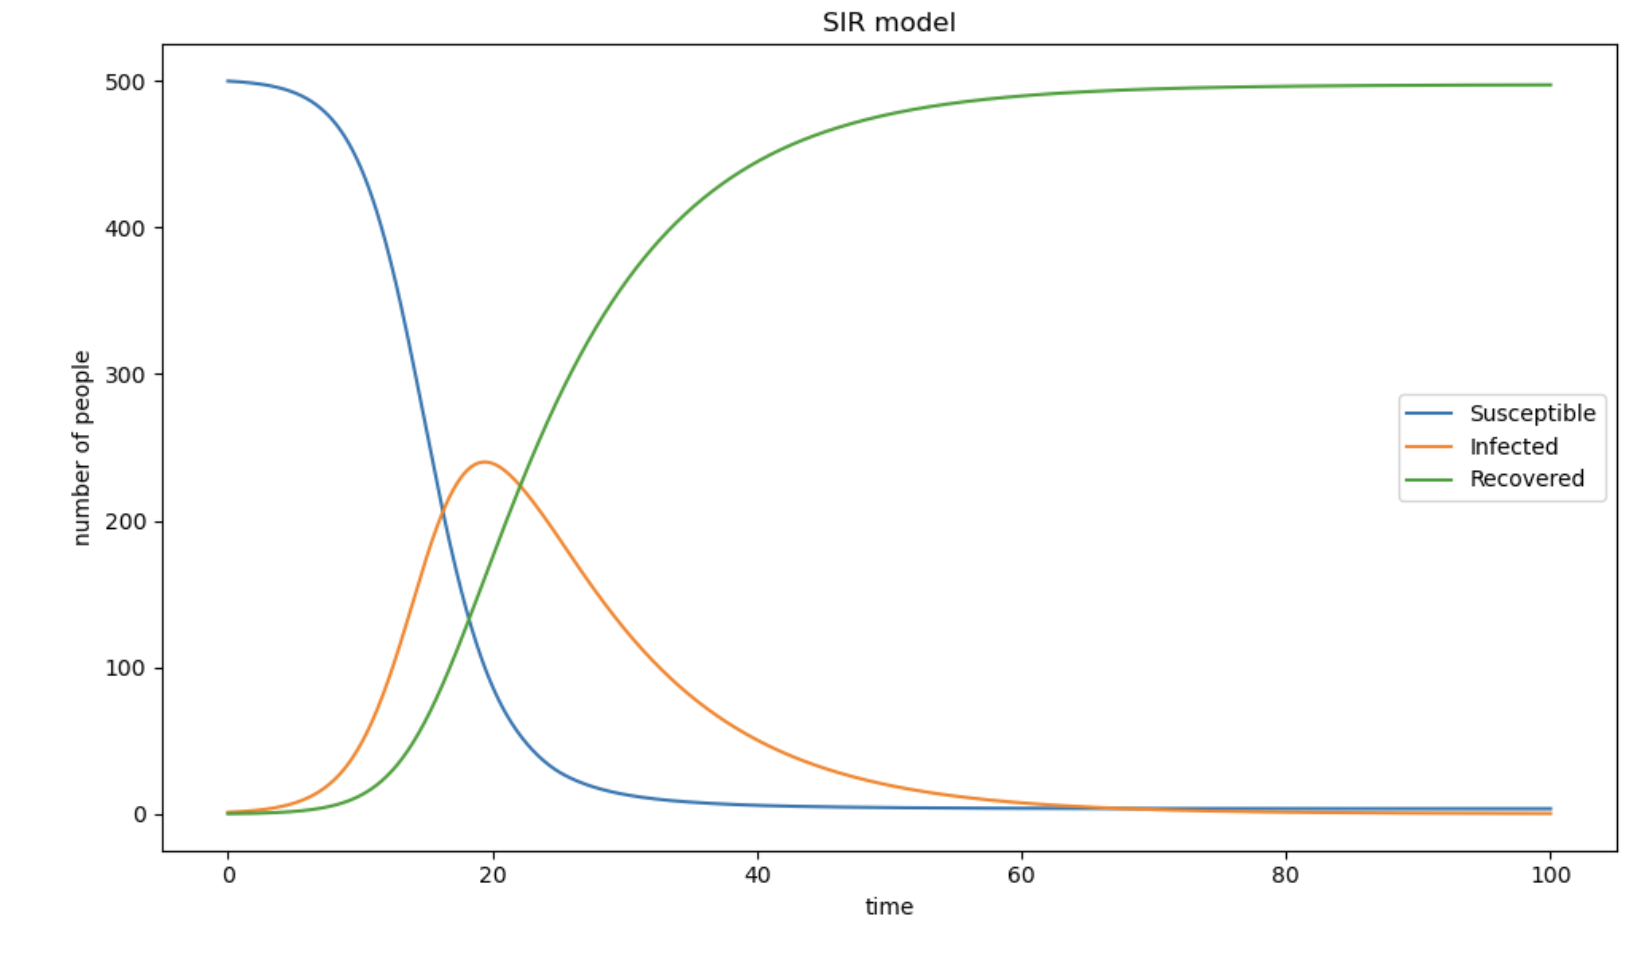
\includegraphics[width=\textwidth]{/Users/ella/edu/uvm25spring/BME3340/L99/media/images/sir-dynamics.png}
        \caption{In the simulation below, we begin with 500 susceptible individuals, 1 infected individual, and plot the dynamics with respect to time.}
        \label{fig:cg}
\end{figure}

The initial susceptible population starts at 500 and decreases with the passage of time. By the end, the number of susceptible people approaches zero because every person will have been infected. Likewise for the recovered population, if everyone has been infected, then recovered, the number of recovered population increases and approaches 500. When the number of susceptible people is greater than the number of recovered, \(\frac{dI}{dt}\) is positive/increasing. As the number of susceptible people drops, the negative term of \(\frac{dI}{dt}\) dominates, and the infected population starts decreasing as they transition to be recovered more quickly than new cases of infection.

We can also explore how changing the transmission rate \(\beta\) affects the dynamics. This models real-world interventions such as social distancing, handwashing, mask-wearing, and other precautions that might slow the spread of disease. Increasing \(\beta\) leads to a faster and more acute outbreak, spreading more quickly and infecting most of the population in a shorter time. Decreasing \(\beta\) causes the outbreak to be more gradual, peaking at a lower level, and spreads over a longer timepsan.

\begin{figure}[h!]
        \centering
        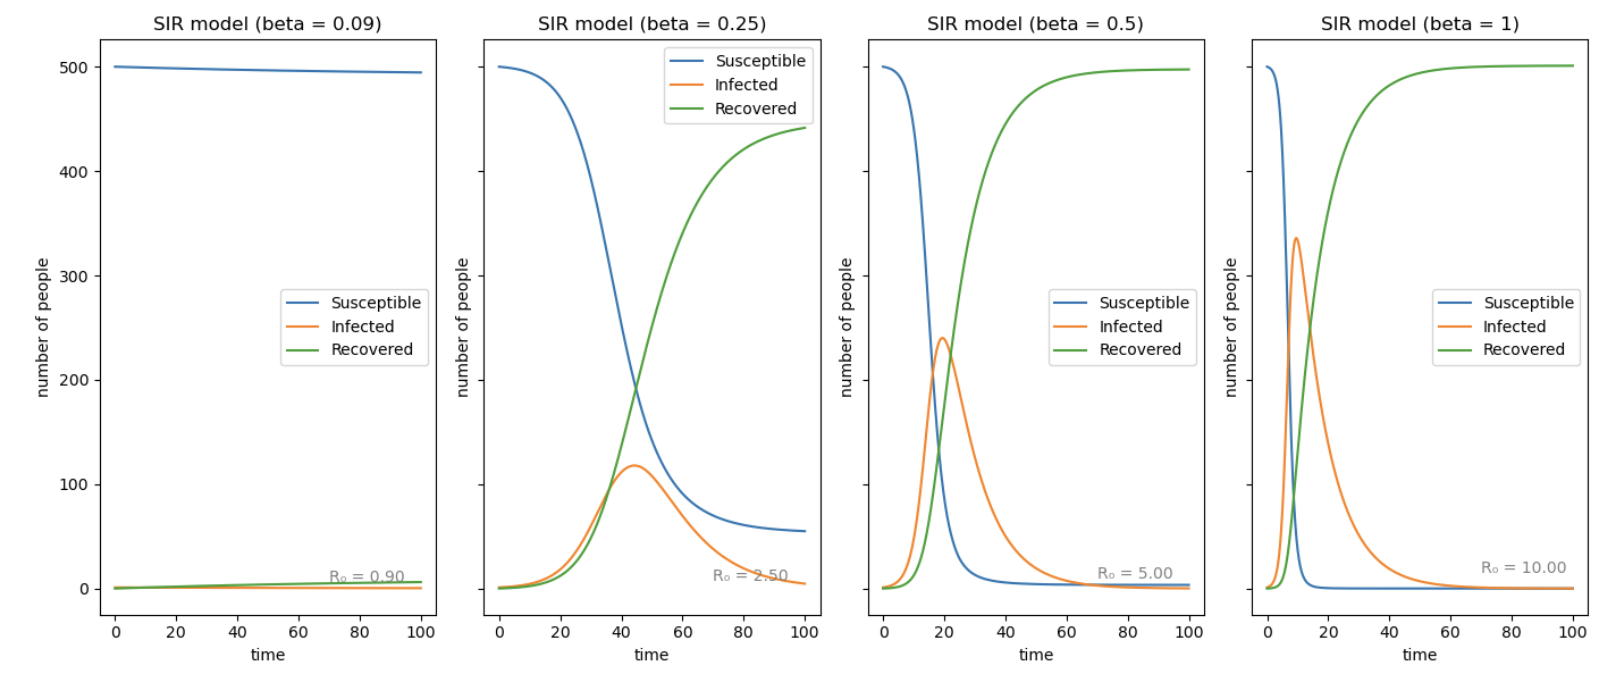
\includegraphics[width=\textwidth]{/Users/ella/edu/uvm25spring/BME3340/L99/media/images/sir-dynamics-with-r.png}
        \caption{SIR dynamics using different values for \(\beta\) and varying results for \(R_0\).}
        \label{fig:cg}
\end{figure}

The basic reproduction number, \( R_0 = \frac{\beta}{\gamma}\), determines whether an outbreak will occur. It represents the expected number of secondary infections caused by one infected individual before they recover (Jones 2021). If \(R_0 > 1\), the number of infected people increases, and an outbreak occurs. If \(R_0 < 1\), the number of infected people does not increase, and there is no epidemic.

Note: \(R_0\) is not to be confused with the initial recovered population \(R(0)\).

\newpage
\section*{Discussion}

In the classical SIR model, infections always die out, and once-infected people are immune indefinitely. These assumptions limit its realism and application to real-world epidemics. For instance, many individuals may lose immunity over time or be reinfected with a mutated strain.  The SEIRS model addresses some of these limitations by extending the SIR model to account for latency using a new group for exposed \(E\) individuals who are infected but not yet infectious, loss of immunity by allowing recovered individuals to become susceptible again, births and deaths to reflect population turnover (Bjornstad and Shea 2020).

In future analysis, the SIR model could be extended to explore spatial models where disease spreads over localized networks or in subpopulations (Ovaskainen and Hanski 2001), or incorporating stochastic effects to account for chance events such as when exactly an individual recovers.

\newpage

\section*{References}
 
 \noindent
Bjørnstad, O.N., Shea, K., Krzywinski, M. et al. 2020. The SEIRS model for infectious disease \\
\indent dynamics. Nat Methods 17, 557–558. https://doi.org/10.1038/s41592-020-0856-2\\

\noindent
Jones, James H. 2021. Notes on R0. Department of Anthropological Sciences, Stanford University.\\ 
\indent https://populationsciences.berkeley.edu/wp-content/uploads/2021/06/Jones-Notes-on-R0.pdf\\

\noindent
Kermack William Ogilvy and McKendrick A. G. 1927 A contribution to the mathematical theory\\
\indent of epidemics Proc. R. Soc. Lond. A115700–721 http://doi.org/10.1098/rspa.1927.0118\\

\noindent
Ovaskainen, O., and I. Hanski. 2001. Spatially structured metapopulation models: Global and \\
\indent local assessment of metapopulation capacity. Theoretical population biology 60:281–302.


\end{document}
